\documentclass[a4paper,12pt]{article}
\usepackage[T2A]{fontenc}
\usepackage[utf8]{inputenc}
\usepackage[top=2cm, bottom=2cm, right=2cm, left=2cm]{geometry}
\usepackage[russian]{babel}
\usepackage{pscyr}
\usepackage{indentfirst}
\usepackage{graphicx}
\usepackage{epstopdf}
\usepackage{amstext}
\usepackage{amssymb}
\usepackage{amsmath}
\usepackage{cmap}
\usepackage{enumitem}
\usepackage{multirow}
\pdfminorversion=6
%\input{environment}
%\linespread{1.3}
\tolerance=1000 
\hfuzz=0pt
\parindent=1.27cm
\usepackage{subcaption}
\captionsetup[table]{name = Таблица, labelsep = endash, justification=raggedright, singlelinecheck=false}
\captionsetup[figure]{name = Рисунок, labelsep = endash}
\usepackage{array}
\usepackage{subcaption}
\usepackage{pgfplots}
\usetikzlibrary{pgfplots.polar}
\pgfplotsset{compat=1.13}
\pgfplotsset{grid = major, grid style = {dashed}}
\usepackage{tabu}
\usepackage{threeparttable}
\usepackage{pgfplotstable}
\renewcommand{\arraystretch}{1.5}
% recommended:
\usepackage{booktabs}
\usepackage{colortbl}


%\sloppy

\graphicspath{{images/}{data/}}


\begin{document}
	\input{page12}
	\paragraph{Цель работы.}  Исследование динамических и частотных характеристик, анализ структурных свойств и устойчивости линейных непрерывных систем с помощью прикладного пакета Matlab Control System Toolbox
	\paragraph {Исходные данные:} Исходная модель разомкнутой системы представляется в форме вход-выход и описывается передаточной функцией вида:\\
	\begin{equation}
	\displaystyle W(s)=\frac{b_1s+b_0}{s(a_2s^2+a_1s+a_0)}
	\end{equation}
	Выберем следующие коэффициенты: $b_1=1, b_0=0, a_2=1, a_1=2, a_0=3$\\
	В итоге передаточная функция примет вид:
	\begin{equation}
	\displaystyle W(s)=\frac{s}{s^3+2s^2+3s}
	\label{eq_1}
	\end{equation}
	\newpage
	\begin{center}
		\section{Анализ исходной разомкнутой системы}
	\end{center}
\subsection{Нули и полюса передаточной функции разомкнутой системы}
Схема расположения нулей и полюсов представлена на рисунке \ref{s_1}.
\begin{figure} [h!]
	\centering
	\begin{tikzpicture}
	\begin{axis} [
	width = 0.8\textwidth,
	xlabel = {Вещественые числа},
	ylabel = {Мнимые числа},
	]
	\addplot[only marks, mark = x, mark size = 5pt] coordinates {(-1, -1.4142) (-1, 1.4142) (0, 0)}; 
	\addplot[only marks, mark = o, mark size = 5pt] coordinates {(0, 0)};
	\legend{Полюса, Нули};
	\end{axis}
	\end{tikzpicture}
	\caption{Схема расположения нулей и полюсов на комплексной плоскости}
	\label{s_1}
\end{figure}

	Данная система находится на апериодической границе устойчивости, т.к один из полюсов(корень характеристического уравнения) равен 0, а остальные имеют отрицательную вещественную часть.
	\newpage
	\subsection{Получение графиков логарифмических амплитудночастотной и фазочастотной характеристик}
	Графики представлены на рисунке \ref{s_2}
	\begin{figure}[h!]
		\begin{subfigure}{\textwidth}
			\centering
			\begin{tikzpicture}
			\begin{semilogxaxis} [
			width = 0.9\textwidth,
			height = 6cm,
			ylabel = {$L(\omega)$, дБ},
			xlabel = {$\omega$, 1/c},
			xmin = 10e-3, xmax = 10e+1,
			xtick = {10e-3, 10e-2, 10e+0, 10e+1},
			ytick = {-10, -20, -40, -60, -80},
			]
			\addplot[blue, mark = none, thick, smooth, solid] table [x = {w}, y = {L}] {data/bode.dat};
			
			\end{semilogxaxis}
			\end{tikzpicture}
		\end{subfigure}
		\begin{subfigure}{\textwidth}
			\centering
			\begin{tikzpicture}
			\begin{semilogxaxis} [
			width = 0.9\textwidth,
			height = 6cm,
			ylabel = {$\psi$, град.},
			xlabel = {$\omega$, 1/c}, 
			xmin = 10e-3, xmax = 10e+1,
			ytick = {0, -90, -180},
			xtick = {10e-3, 10e-2, 10e+0, 10e+1},
			]
			\addplot [blue, mark = none, thick, smooth, solid] table [x = {w}, y = {ugol}] {data/bode.dat};
			\end{semilogxaxis}
			\end{tikzpicture}
		\end{subfigure}
		\caption{ЛАЧХ и ЛФЧХ}
		\label{s_2}
	\end{figure}
	\\
	Запас устойчивости по амплитуде, как и по фазе, бесконечный.
	\newpage
	\subsection{Построение амплитуднофазочастотной характеристики системы}
	График представлены на рисунке \ref{s_3}.
	\begin{figure}[h!]
		\begin{center}
			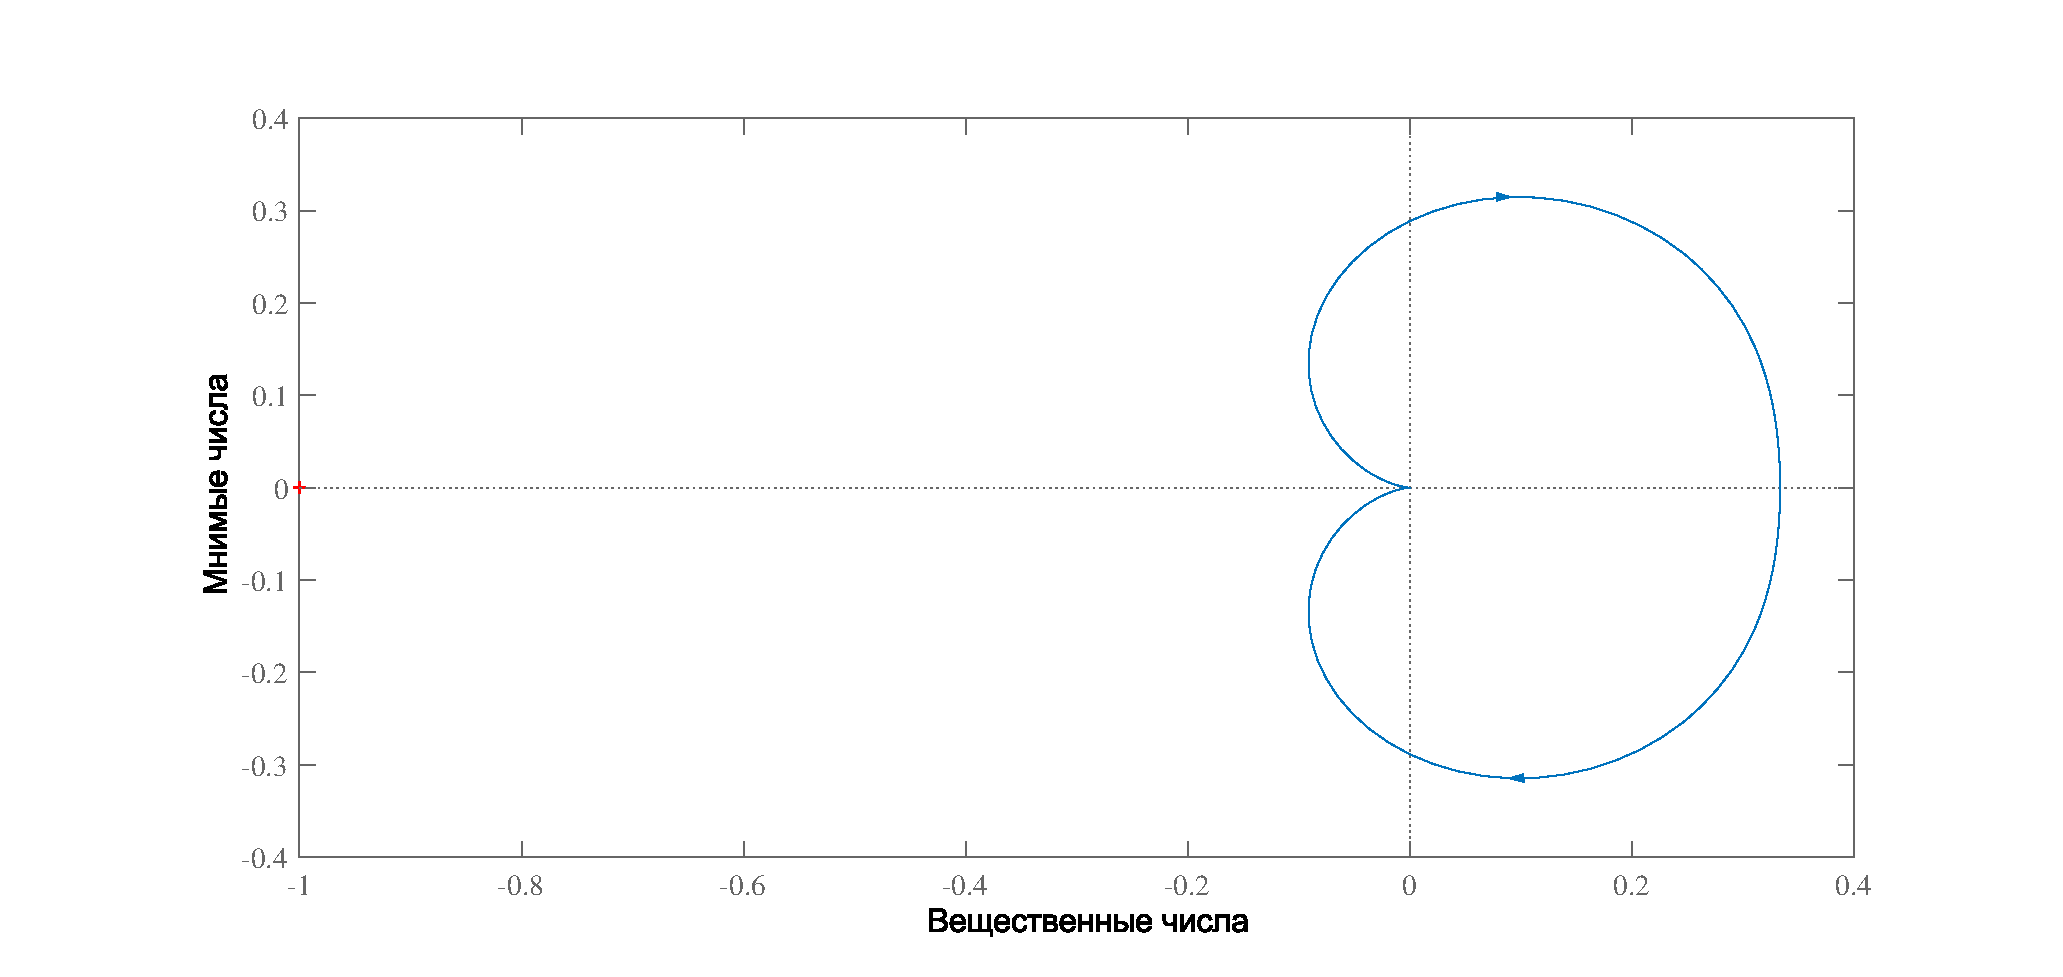
\includegraphics[width=7in]{nyquist.eps}
			
		\end{center}
	\caption{Диаграмма Найквиста}
	\label{s_3}  
	\end{figure}
	\\
	По критерию	Найквиста система устойчива, так как точка (-1,0j) не охватывается.
	
		
	\newpage
	\begin{center}
		\section{Анализ замкнутой системы}
	\end{center}
	\subsection{Анализ влияния коэффициентов обратной связи на устойчивость замкнутой системы и схема расположения нулей и полюсов системы}
	После охватывания системы (\ref{eq_1}) обратной связью с коэффициентом $K$ получившаяся замкнутая система имеет передаточную функцию вида:\\
	
	\begin{equation}
	\displaystyle W(s)=\frac{s}{s^3+2s^2+s(3+K)}
	\label{eq_2}
	\end{equation}\\
	
	\par 
	Анализируя эту функцию на устойчивость по критерию Гурвица можно сделать вывод, что данная система находится на апериодической границе устойчивости, т.к свободный член характеристического полинома тождественно равен нулю. А для того, чтобы система не выходила за границы устойчивости, требуется, чтобы $K\ge-3$
	%\newpage
	\par
	Выберем $K=-1$. Тогда передаточная функция системы будет равна:
	\begin{equation}
	\displaystyle W(s)=\frac{s}{s^3+2s^2+2s}
	\label{eq_3}
	\end{equation}
	Схема расположения нулей и полюсов представлена на рисунке \ref{s_4}.
	\begin{figure} [h!]
		\centering
		\begin{tikzpicture}
		\begin{axis} [
		width = 0.8\textwidth,
		xlabel = {Вещественые числа},
		ylabel = {Мнимые числа},
		]
		\addplot[only marks, mark = x, mark size = 5pt] coordinates {(-1, -1) (-1, 1) (0, 0)}; 
		\addplot[only marks, mark = o, mark size = 5pt] coordinates {(0, 0)};
		\legend{Полюса, Нули};
		\end{axis}
		\end{tikzpicture}
		\caption{Схема расположения нулей и полюсов на комплексной плоскости}
		\label{s_4}
	\end{figure} 
	
	Степень устойчивости системы $\eta$ - абсолютное значение вещественной части ближайшего к мнимой оси корня. В данном случае $\eta$=0 

	\newpage
	\subsection{Получение графика переходной и весовой функций замкнутой системы}
	График переходной функции представлен на рисунке \ref{s_5} 
	\begin{figure}[h!]
		\begin{center}
			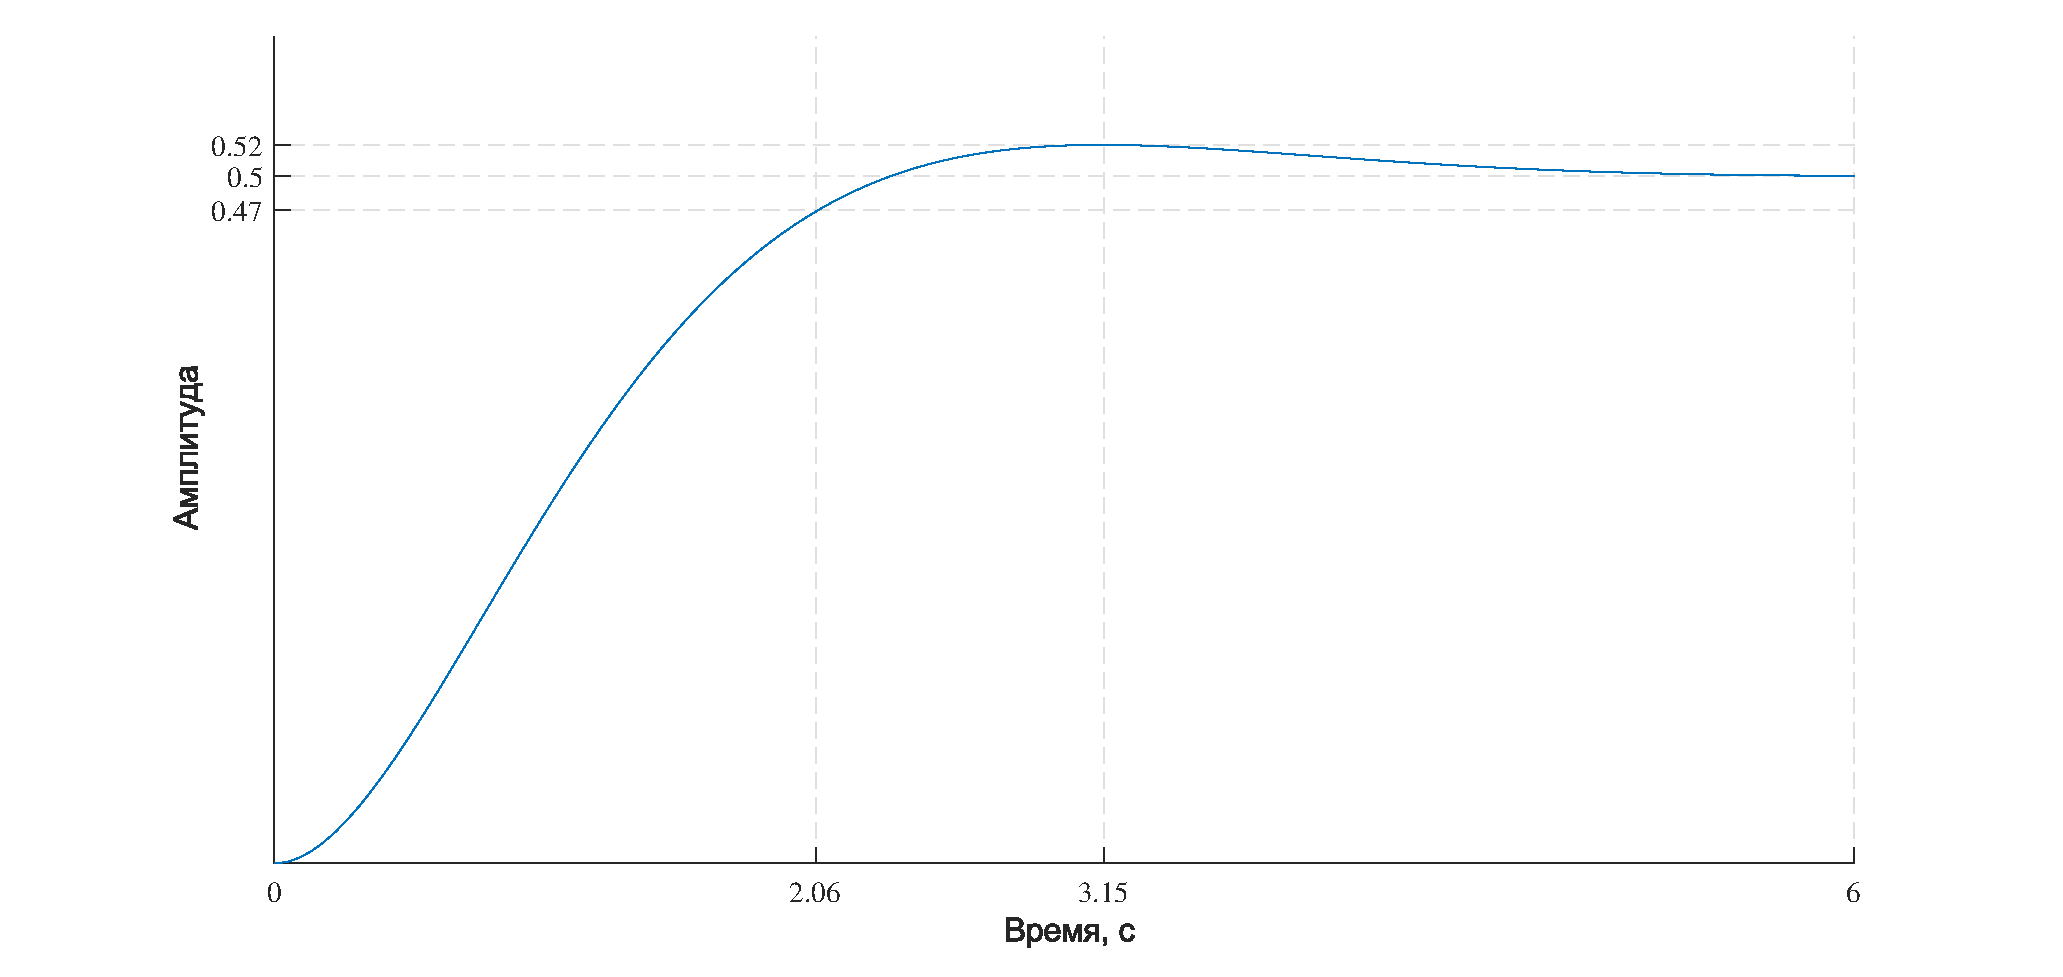
\includegraphics[width=7in]{pereh.eps}
			
		\end{center}
		\caption{Переходная функция}
		\label{s_5}  
	\end{figure}
	
	Перерегулирование $\sigma=4$\%, Время переходного процесса $t_\text{п}=2.06$с \\

График весовой функции представлен на рисунке \ref{s_5} 
\begin{figure}[h!]
	\begin{center}
		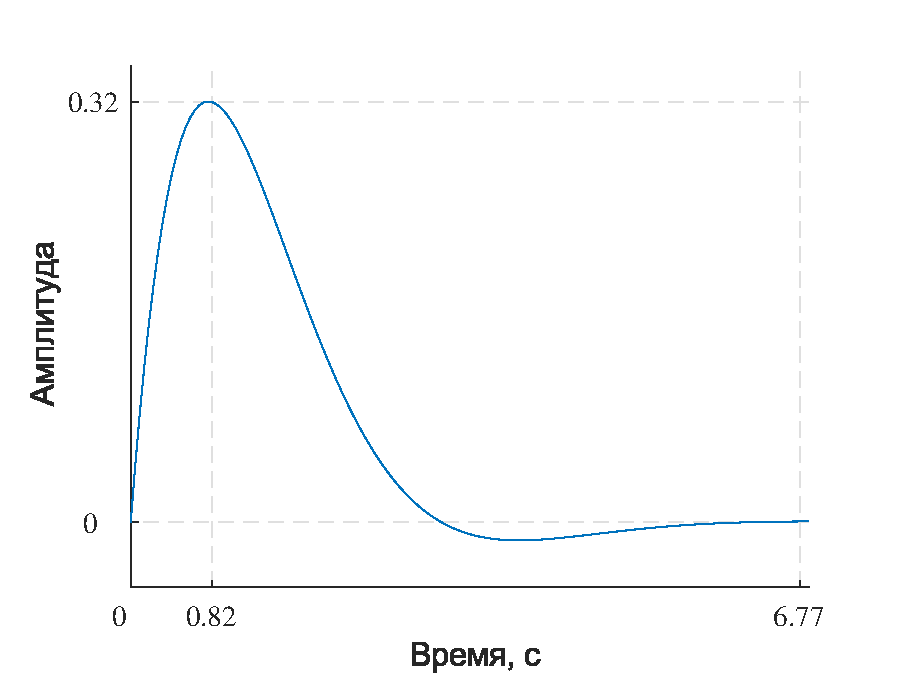
\includegraphics[width=5in]{ves.eps}
		
	\end{center}
	\caption{Весовая функция}
	\label{s_6}  
\end{figure}
	
	\newpage
	\subsection{Переход к представлению замкнутой системы в форме ВСВ}
	Дифференциальное уравнение, описывающее систему имеет вид:\\
	\begin{equation}
	\dot{g}=\dddot{y}+2\ddot{y}+2\dot{y}
	\end{equation}
	Представим систему в матричной форме:\\
	\begin{equation}
	\begin{cases}
	\dot{X}=A\cdot X + B\cdot u 
	\\
	y = C\cdot X + D\cdot u
	\end{cases}
	\end{equation}
	Возьмем в качестве вектора состояния $X=\begin{bmatrix}
	y & \\
	\dot{y} &\\
	\ddot{y} 
	\end{bmatrix}$
	а за вектор возмущающих воздействий $u=\begin{bmatrix}
	0 \\
	0 \\
	\dot{g}\\ \end{bmatrix}$ \\
	\noindent Выходная величина $y=y ~\Rightarrow~ C=\begin{bmatrix}
	1 & 0 & 0 \\ \end{bmatrix} ~~D=0$ \\
	Матрицы $A$ и $B$ тогда равны:\\ 
	\begin{gather}
	\displaystyle A=\begin{bmatrix}
	 0 & 1 & 0\\
	0 & 0 & 1\\
	0 & -2 & -2\\
	\end{bmatrix} 
	\\ B=\begin{bmatrix}
	0 \\
	0 \\
	1\\
	\end{bmatrix}
	\end{gather}
	Оценим управляемость и наблюдаемость системы.\\
	Матрица управляемости:\\
	\begin{gather}
	\displaystyle K_y=\begin{bmatrix}
	0 & 0 & 1\\
	0 & 1 & -2\\
	1 & -2 & 2\\
	\end{bmatrix} 
		\end{gather}
		Матрица наблюдаемости:\\
	
	\begin{gather}
	\displaystyle K_\text{н}=\begin{bmatrix}
	1 & 0 & 0\\
	0 & 0 & 0\\
	0 & 0 & 0\\
	\end{bmatrix} 
		\end{gather}
	
	Так как $rank(K_y)=3$ а $rank(K_{\text{н}})=1$ то система является только полностью управляемой.
	
	\newpage
	\begin{center}
		\section*{Вывод}
	\end{center}
	\par
	В данной работе с помощью пакета Matlab Control System Toolbox был проведен анализ разомкнутой и замкнутой систем. Были найдены полюса и нули характеристических уравнений для обеих систем и отображены на комплексную плоскость, по которым можно судь об устойчивости системы, также были получена диаграмма Найквиста, которая показывает устойчивость системы, и ЛАЧХ и ЛФЧХ, по которым можно определить устойчивость по фазе и амплитуде.
	\par
	Для замкнутой системы были получены переходная и весовая функции и определены значения перерегулирования и времени переходного процесса. Также система была представлена в матричной форме, для который  были найдены матрицы управляемости и наблюдаемости.
	
\end{document}